% Created 2015-10-27 二 19:48
\documentclass[11pt]{article}
\usepackage[utf8]{inputenc}
\usepackage[T1]{fontenc}
\usepackage{fixltx2e}
\usepackage{graphicx}
\usepackage{longtable}
\usepackage{float}
\usepackage{wrapfig}
\usepackage{rotating}
\usepackage[normalem]{ulem}
\usepackage{amsmath}
\usepackage{textcomp}
\usepackage{marvosym}
\usepackage{wasysym}
\usepackage{amssymb}
\usepackage{hyperref}
\tolerance=1000
\usepackage{xeCJK}
\usepackage{framed}
\author{钱泽森(5130379069)}
\date{\today}
\title{Quidditch桌球详细设计说明书}
\hypersetup{
  pdfkeywords={},
  pdfsubject={},
  pdfcreator={Emacs 24.5.1 (Org mode 8.2.10)}}
\begin{document}

\maketitle
\tableofcontents


\section{引言}
\label{sec-1}
\subsection{编写目的和范围}
\label{sec-1-1}
本详细设计说明书编写的目的是说明程序模块的设计考虑,包括程序描述、
输入/输出、算法和流程逻辑等,为软件编程和系统维护提供基础。本说明书
的预期读者为系统设计人员、软件开发人员、软件测试人员和项目评审人员。
\subsection{术语表}
\label{sec-1-2}
\begin{description}
\item[{Buffer Object}] An object that represents a linear array of
memory, which is stored in the GPU. There are
numerous ways to have the GPU access data in a
buffer object.
\item[{Context, OpenGL}] A collection of state, memory and resources.
Required to do any OpenGL operation.
\item[{OpenGL Shading Language}] The language for writing Shaders in
OpenGL.
\item[{Shader}] A program, written in the OpenGL Shader Language,
intended to run within OpenGL.
\item[{Texture}] An OpenGL object that contains one or more images, all
of which are stored in the same Image Format.
\item[{OpenGL}] A cross-platform graphics system with an openly
available specification.
\end{description}
\subsection{参考资料}
\label{sec-1-3}
\begin{center}
\begin{tabular}{llll}
资料名称 & 作者 & 文件编号/版本 & 资料存放地点\\
OpenGL Tutorial & Unknown & latest & \url{http://www.opengl-tutorial.org}\\
OpenGL step by step & Unknown & Latest & \url{http://ogldev.atspace.co.uk/}\\
OpenGL wiki & collabrators & Latest & \url{https://www.opengl.org/wiki/}\\
OpenGL 3.3 Reference Pages & SGI & 3.3 & \url{https://www.opengl.org/sdk/docs/}\\
\end{tabular}
\end{center}

\subsection{使用的文字处理和绘图工具}
\label{sec-1-4}
\begin{description}
\item[{文字处理软件}] Emacs, Org Mode
\item[{UML图生成}] Doxygen
\end{description}
\section{技术概要}
\label{sec-2}
\begin{itemize}
\item 基于OpenGL 3.3 core API
\item 使用了 SFML 作为window system
\item 使用 glew 作为Extension Wrangler Library
\item 使用glm作为数学库
\item 开发环境为Linux x86-64 + Mesa
\end{itemize}
\section{模块设计}
\label{sec-3}
\subsection{用例图}
\label{sec-3-1}
\begin{figure}[h]
 \centering
 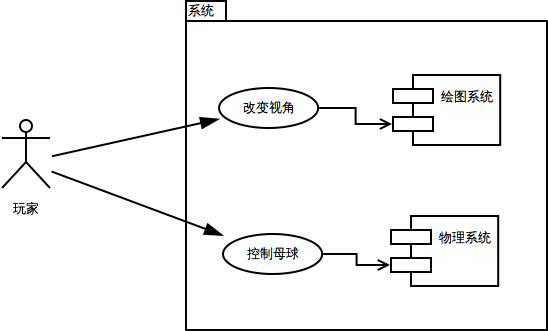
\includegraphics[width=0.8\textwidth]{usecase.png}
 \caption{用例图}
 \label{fig:usecase}
 \end{figure}
\subsection{功能设计说明}
\label{sec-3-2}
\subsubsection{物理模块}
\label{sec-3-2-1}
物理模块主要由沙盒(Arena)和各个物理元件(SnitchBall, GhostBall,
CueBall, WanderBall, Wall)构成. 
\begin{enumerate}
\item 沙盒(Arena)
\label{sec-3-2-1-1}
沙盒模块负责对物理世界进行仿真模拟, 它负责的物理模拟主要有以下几
类:
\begin{description}
\item[{滚动摩擦}] 在桌面上的小球在不受到其他外力的情况下, 会收到桌布
的滚动摩擦力, 因此速度会越来越小.
\item[{小球间碰撞}] 小球之间会产生非弹性碰撞, 碰撞后两球的速度和方向
都会发生变化, 此过程会有能量损失.
\item[{小球和桌面以及墙面的碰撞}] 小球和桌面以及墙面也会产生非弹性碰
撞.
\end{description}

沙盒每次都往前演绎一段时间, 并且不断修改球桌上元件的物理属性, 来
反映物理世界的规律.
\item 球(Ball)
\label{sec-3-2-1-2}
所有球类的父类, 主要记录球的质量/半径/位置/速度. Ball的继承关系请
见 \ref{fig:ball_inherit}.
\begin{figure}[h]
\centering
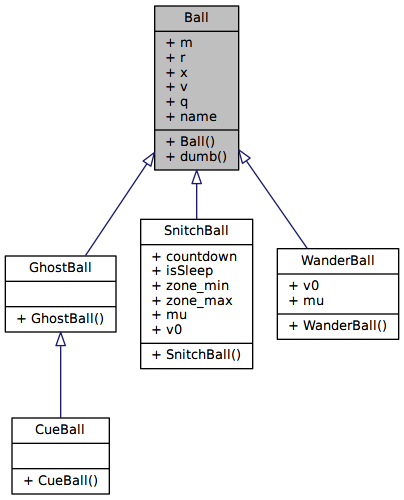
\includegraphics[width=0.8\textwidth]{html/struct_ball__inherit__graph.png}
\caption{Ball的继承关系}
\label{fig:ball_inherit}
\end{figure}
\item 幽灵球(GhostBall)
\label{sec-3-2-1-3}
普通球, 直接继承自Ball, 没有额外的属性. 
\item 母球(CueBall)
\label{sec-3-2-1-4}
用户可以操作的球, 继承自GhostBall, 没有额外的属性.
\item 游走球(WanderBall)
\label{sec-3-2-1-5}
自主随机游走的球, 继承自Ball. 额外属性: v0表示理想速度, mu表示趋
近速度. 在当前速度不等于理想速度时, 本球会以mu的速率逐渐趋近于v0.
\item 金色飞贼(SnitchBall)
\label{sec-3-2-1-6}
会飞的球. 继承自Ball, 需要额外记录当前状态下剩余的时间(以秒表示),
以及理想的飞行速度.

\item 墙(Wall)
\label{sec-3-2-1-7}
表示沙盒的边缘, 既可以用来表示垂直的墙, 也可以表示地面或者天花板.
属性有: 一次方程的一组参数, 用来表示墙的平面. 以及一个弹性系数,
用来表示球和墙碰撞后的能量损失程度.
\end{enumerate}
\subsubsection{绘图模块}
\label{sec-3-2-2}
绘图模块主要负责在屏幕上绘图.
\begin{enumerate}
\item 可渲染物体(Renderable)
\label{sec-3-2-2-1}
定义了一个通用接口, 调用后即会画出该物体. 
\item 视角(View)
\label{sec-3-2-2-2}
表示用户的视角, 包括摄像头所在的位置, 观察的方向等等, 可以调用获
取对应的View Matirx.
\item 投影(Projection)
\label{sec-3-2-2-3}
表示摄像头的投影, 包括横向的和纵向的视角, 最近的切点和最远处的切
点, 可以调用获取对应的Projection Matrix.
\item 场景(Scene)
\label{sec-3-2-2-4}
表示一个完整的场景, 包括一些Renderable, 一个View, 一个Projection.
调用后即会画出整个场景.
\item 形状(Shape)
\label{sec-3-2-2-5}
表示一个固定的形状, 比如, 处在原点且半径为1的球, 或者处在原点且边
长为1的立方体, 等等.
\end{enumerate}
\subsubsection{接口模块}
\label{sec-3-2-3}
接口模块主要用来衔接物理模块和绘图模块.
\begin{enumerate}
\item BallWrapper
\label{sec-3-2-3-1}
一个包装类, 是Renderable的子类. 主要用来将Ball的物理属性, 转化为Renderable的绘图属性.
比如, 如果Ball的x属性是(1, 0, 0), 则生成的Renderable会在(1, 0,
0)处画一个球.
\item Table
\label{sec-3-2-3-2}
一个包装类, 是Renderable的子类. 主要用来将Arena的物理属性, 转化为
renderable的绘图属性.
\end{enumerate}
\subsubsection{控制模块}
\label{sec-3-2-4}
负责读取用户的输入并且修改对应的游戏状态. 比如鼠标移动, 则修改
View的相关属性, 等等.
\section{接口设计}
\label{sec-4}
\subsection{内部接口}
\label{sec-4-1}
\subsubsection{Shape}
\label{sec-4-1-1}

\texttt{virtual void draw() const}

调用即绘出这个形状.


\subsubsection{Renderable}
\label{sec-4-1-2}

\texttt{virtual void render(const GLuint WVP, const glm::mat4 \&mat) const}
\begin{description}
\item[{WVP}] World-View-Projection矩阵所对应的Uniform Variable编号
\item[{mat}] 已经算出的View-Projection矩阵
\end{description}

调用后, Renderable会计算出最终的WVP并且绑定, 最终绘出该物体.

\subsubsection{Arena}
\label{sec-4-1-3}

\texttt{void deduce(const float t)}
\begin{description}
\item[{t}] 距离上次调用逝去的时间,单位为秒
\end{description}
调用后, Arena会推算物体运动并且修改响应的物体的状态.



\texttt{void attach(Ball *ball)}
\begin{description}
\item[{ball}] 需要添加的球
\end{description}



\texttt{void attach(Wall *wall)}
\begin{description}
\item[{wall}] 需要添加的墙
\end{description}

\subsubsection{Scene}
\label{sec-4-1-4}

\texttt{Scene(const View \&view, const Projection \&projection)}
\begin{description}
\item[{view}] 观察该场景的视角
\item[{projection}] 观察该场景的投影
\end{description}


\texttt{void render()}

调用即绘出这个场景.

\texttt{void attach(Renderable * renderable)}
\begin{description}
\item[{renderable}] 需要添加的物体
\end{description}
\section{系统性能设计}
\label{sec-5}
为了性能考虑, 本软件使用OpenGL 3.3 Core API, 避免了大量的
\texttt{glBegin()} 和 \texttt{glEnd()} 调用, 极大地提高了性能.  
\section{系统出错处理}
\label{sec-6}
本系统可能遇到的错误有以下几类
\begin{description}
\item[{载入纹理错误}] 致命错误, 程序直接退出
\item[{载入音效错误}] 致命错误, 程序直接退出
\item[{其他错误}] 输出到终端, 不影响程序运行
\end{description}
% Emacs 24.5.1 (Org mode 8.2.10)
\end{document}